\section{Using new techniques for VBF H(inv) analysis}

\graphicspath{{5_Outlook/Figures}}

In addition to the detector-related upgrades mentioned in the previous sections, search for novel techniques
to improve the sensitivity of the VBF $\hinv$ analysis are also underway. In the analysis methodology described
in this thesis, kinematic variables of two outgoing VBF jets were used to distinguish VBF $\hinv$ signal from
most of the SM backgrounds. An interesting line of development related to the goal of increasing the sensitivity 
of the analysis is the use of new machine learning (ML) techniques, in an attempt to develop classifiers to
more efficiently classify signal from SM background. One important example of such a classifier is called
ParticleNet~\cite{CMS:ParticleNetPaper}. 

ParticleNet is a graph neural network which takes lower-level point-like
objects as input, for example the set of particles reconstructed within the event. It treats all particles
as a ``point cloud'' data structure, which is a permutationally invariant set of points each carrying a feature
vector, composed of features such as $\pt$, $\eta$, $\phi$ and so on. ParticleNet then applies the edge convolution
(EdgeConv) operation~\cite{Wang:DynamicGraphCNNPaper} on the point-cloud data structure. This operation can be
understood as a convolution-like operation for point clouds, where the point cloud data structure is treated as
a graph, where each point is a vertex, and connections between points represent edges. For each vertex, $k$
nearest neighbors can be identified. The EdgeConv operation for each point $x_{i}$ then has the form

\begin{equation}
    \mathbf{x_i'} = \frac{1}{k} \sum_{j=1}^{k} h_{\Theta}(\mathbf{x_i}, \mathbf{x_{j_i}})
\end{equation}

where $\mathbf{x_i}$ denotes the feature vector of the point $x_i$ and ${i_1,...,i_k}$ are the indices of the 
$k$-nearest neighbors of $x_i$. The edge function $h_{\Theta}$ is some function that is parametrized by
a set of learnable parameters, $\Theta$. It should also be noted that this EdgeConv operation is stackable,
just as a regular convolution operation. This is because EdgeConv is essentially a mapping between an input
point cloud to another point cloud with the same number of points with updated feature vectors. 
This allows to build a deep neural network architecture 
using stacked EdgeConv operations, which can learn features of point clouds 
hierarchically~\cite{CMS:ParticleNetPaper}. 
This feature is exploited in the ParticleNet model architecture, which is shown in Fig.~\ref{fig:particlenet_arch}.

\begin{figure}[htbp]
    \centering
    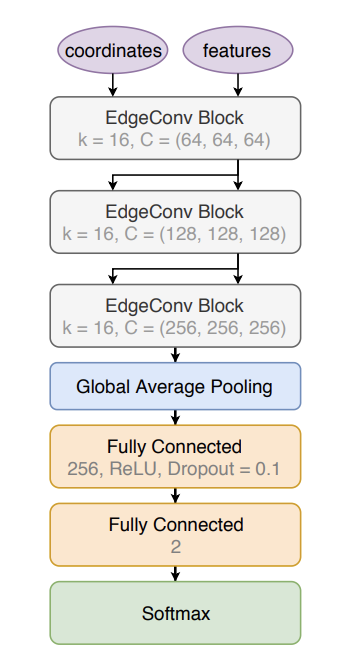
\includegraphics[width=0.3\textwidth]{VBFML/particlenet_arch.png}
    \caption{Architecture of the ParticleNet model. Three EdgeConv operations are stacked together
    with the number of nearest neighbors is taken to be $k=16$. Afterwards, a global average pooling
    is applied to aggregate the learned features over all particles in the cloud, which is followed
    with a densely connected network. A softmax function is used to compute the output for the binary
    classification task. Figure is taken from~\cite{CMS:ParticleNetPaper}.}
    \label{fig:particlenet_arch}
\end{figure}

\subsection{Applying ParticleNet to develop a VBF-tagger}

ParticleNet architecture can be used to develop a classifier with the goal of distinguishing VBF $\hinv$ signal events
from other Higgs production mechanism modes, such as gluon-gluon fusion ($\ggh$). 
To classify a given event as such, the set of particles reconstructed
in the event can be fed into the ParticleNet model, with the list of $[\eta, \phi]$ coordinates for each particle, and their feature
vectors specifying their energy, $\pt$, electrical charge and so on. The aim is to achieve this classification using the hadronic
activity in the events (i.e. the two energetic VBF jets, and potentially softer jets coming from NLO effects), therefore any
reconstructed lepton or photon particle within the event is discarded from the set of input particles. This has profound importance
when the tagger is applied to SM processes such as $\Wlvjets$ to predict whether it is kinematically ``gluon-fusion like'' or ``VBF-like''.

Such a ParticleNet-based VBF classifier, trained on events with gluon-fusion and VBF Higgs production,
is tested by applying the model to classify simulated events within the VBF signal region phase space,
as described in Sec.~\ref{sec:event_selection}. A distribution of score values for different types of Higgs production events is shown in
Fig.~\ref{fig:score_distribution_hinv_events}. It can be observed that VBF $\hinv$ events are accumulated at higher score values, while all the
other Higgs production events have a flat distribution as a function of the ParticleNet score.

To quantify the performance of the ParticleNet-based classification, and compare it with predictions made by different $\mjj$ cuts, the
receiver-operator characteristic (ROC) curve can be calculated for both scenarios and those can be compared. These ROC curves are shown in
Fig.~\ref{fig:ggh_vs_vbfh_roc}. Here, the blue curve corresponds to the ParticleNet-based VBF classifier, and the orange curve corresponds
to a purely $\mjj$-based classifier, which corresponds to the true positive and false
positive event fractions when different $\mjj$ cuts are applied. It can be observed from the area under the ROC curves (AUC), the ParticleNet-based 
classifier performs better than a purely $\mjj$-based classifier.

It is also interesting and instructive to study the event features which are correlated with the ParticleNet prediction. Fig.~\ref{fig:ggh_dnn_event_kinematics},
shows kinematic distributions of the two final-state jets for the $\ggh$ events, where the events are categorized into two: Events correctly classified as
being ``gluon-fusion like'' (hence, DNN score $<0.5$), and events classified as ``VBF-like''. The first plot in Fig.~\ref{fig:ggh_dnn_event_kinematics}
shows the $\Delta\eta_{jj}$ between the two final state jets, and the second plot shows the $\eta$ of the second (trailing in $\pt$) jet. 
It can be observed that the presence of a forward jet in the event (with higher $\eta$) increases the probability of that event being classified as ``VBF-like''.
From the $\Delta\eta_{jj}$ plot on Fig.~\ref{fig:ggh_dnn_event_kinematics}, it can be observed that almost all $\ggh$ events with $\Delta\eta_{jj} > 5$ are
classified as ``VBF-like''. This is however not an unexpected feature, because of the event topology of VBF $\hinv$ events with forward final-state jets,
which is learned by the model during the training phase. This however, makes it more challenging to classify SM backgrounds that originate from VBF processes,
such as the electroweak production of $\Zvvjets$ or $\Wlvjets$, where forward jets also appear in the final state.

\begin{figure}[htbp]
    \centering
    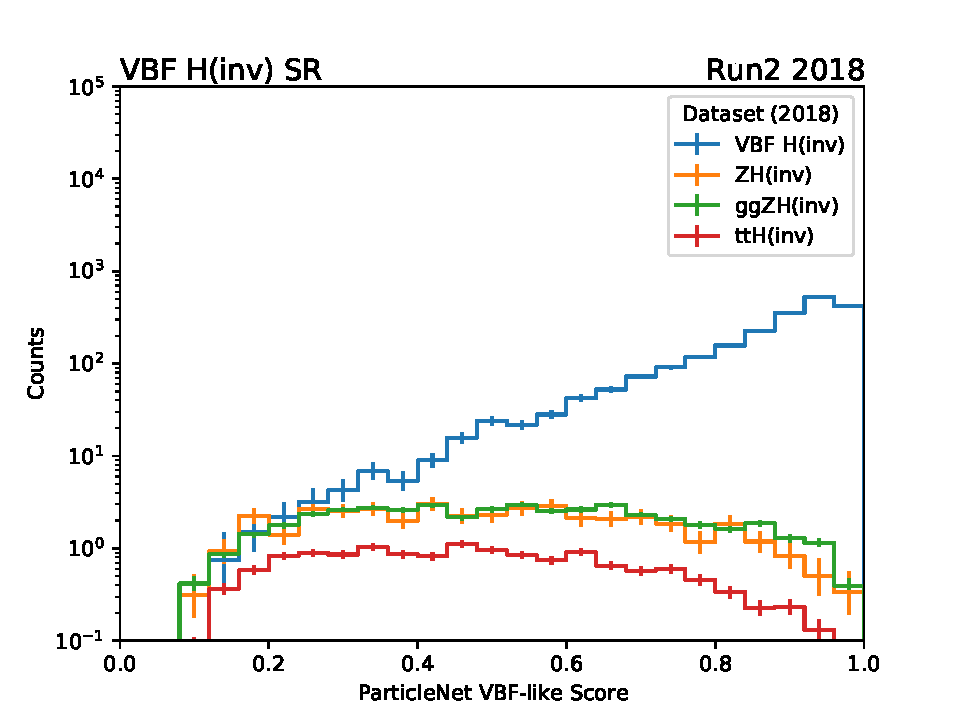
\includegraphics[width=0.8\textwidth]{VBFML/sr_vbf_no_veto_all_particlenet_score.pdf}
    \caption{VBF-tagger score distribution for different types of Higgs production events that pass the VBF signal region selection.
    It can be observed that the VBF $\hinv$ shape is accumulated at higher score values, while all the other Higgs production events
    have a flat distribution.}
    \label{fig:score_distribution_hinv_events}
\end{figure}

\begin{figure}[htbp]
    \centering
    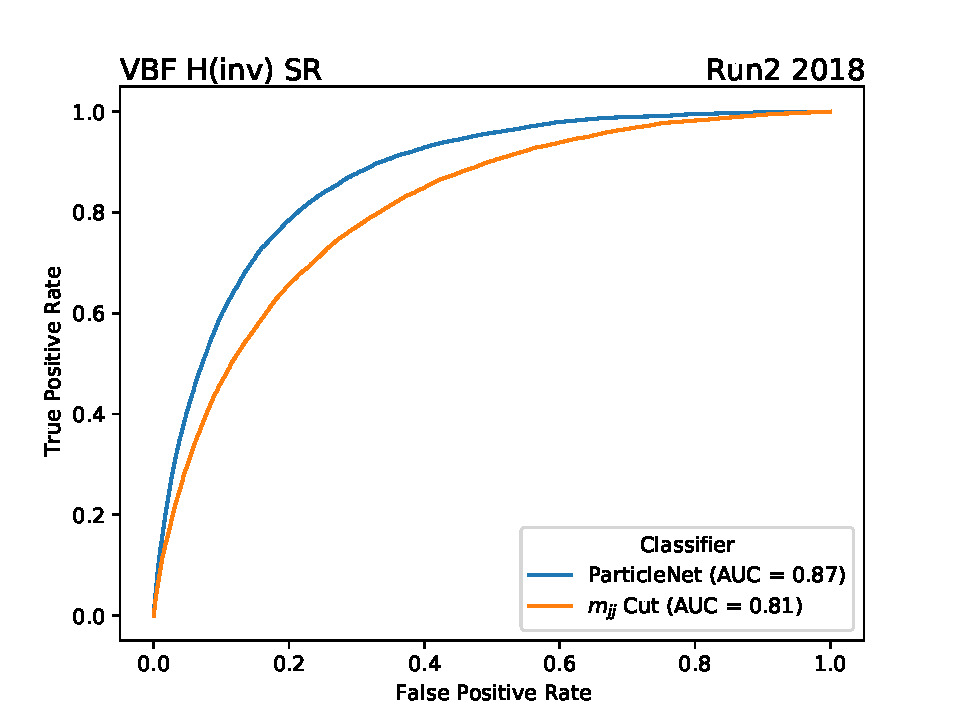
\includegraphics[width=0.8\textwidth]{VBFML/ggH_vs_vbfH_ROC.pdf}
    \caption{Receiver-operator characteristic (ROC) curve for the classification of $\ggh$ and VBF $\hinv$ events that pass the VBF signal region
    selection. The blue curve shows the ROC curve for the ParticleNet-based classifier, while the orange curve shows the ROC curve for the case
    of different $\mjj$ cuts being applied to label events. It can be observed that the ParticleNet classifier performs better than purely $\mjj$-
    based event discirmination. Area under the ROC curve (AUC) is also provided in the legend for the two ROC curves.}
    \label{fig:ggh_vs_vbfh_roc}
\end{figure}

\begin{figure}[htbp]
    \centering
    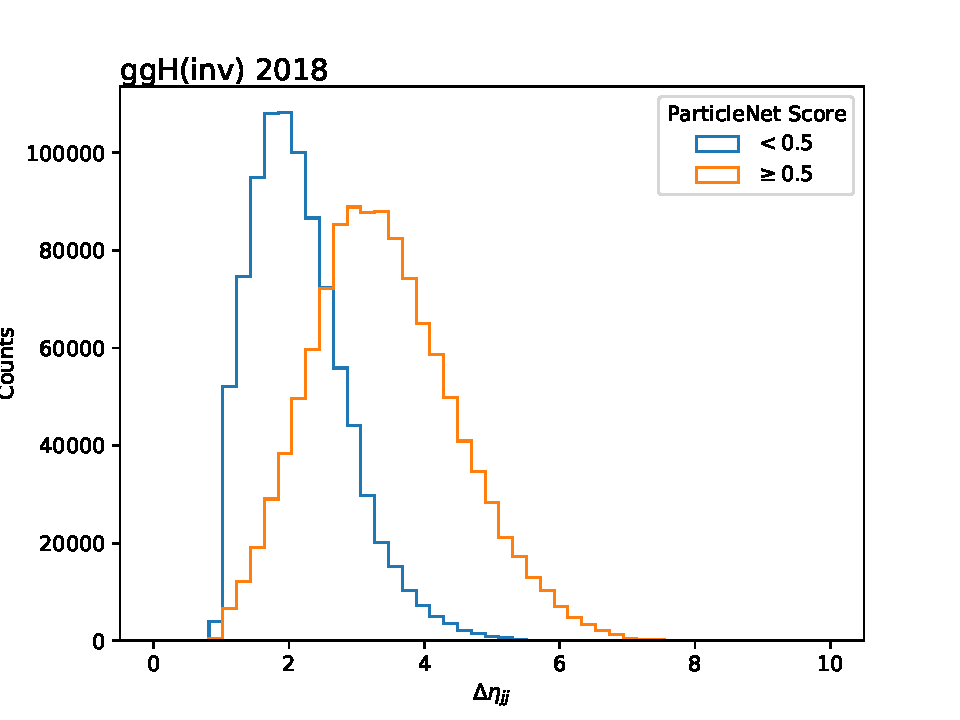
\includegraphics[width=0.45\textwidth]{VBFML/ggH_score_overlayed_detajj.pdf}
    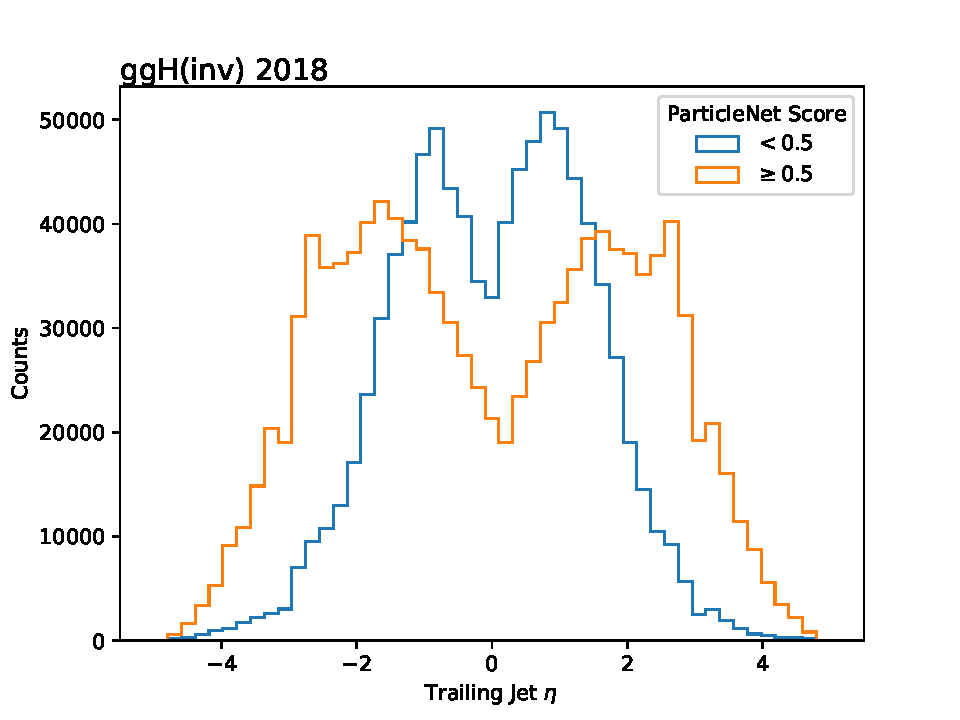
\includegraphics[width=0.45\textwidth]{VBFML/ggH_score_overlayed_trailak4_eta.pdf}
    \caption{$\Delta\eta_{jj}$ between the two final state jets (left) and $\eta$ of the trailing jet (right) for $\ggh$ simulation events. 
    The events are categorized into two,
    where the first group (blue) is classified as ``gluon-fusion-like'' and the second group (orange) is classified as ``VBF-like''. It can be observed
    that the presence of a forward jet is correlated with the score output of the VBF classifier, making it more probable 
    that the event will be classified as VBF-like.}
    \label{fig:ggh_dnn_event_kinematics}
    
\end{figure}

\clearpage

\subsection{Preliminary results}

At the time of writing of this thesis, the application of this ParticleNet based VBF-tagger to the VBF $\hinv$ analysis is preliminary, and final
results with the fit to full Run2 dataset has not yet been obtained. However, some preliminary results will be shown in this section in an attempt
to display the work done so far, and provide a basis of discussion for the potential future work.

One aim of the studies done so far is to apply the VBF-tagger to classify events in proton-proton collision data, and see if the tagger can provide
similar performance of event classification in data and simulation. For this purpose, 2018 dataset is used, and the regular analysis selection
(described in Sec.~\ref{sec:event_selection}) is applied. To test the agreement between data and simulation as a function of the VBF-tagger score,
data in control regions are used. For the purposes of this study, minor backgrounds such as top quark and diboson production are ignored.
Fig.~\ref{fig:single_lep_crs_vbfml} shows the data-to-simulation agreement as a function of the VBF-tagger score for the $Z$ and $W$ control regions.

\begin{figure}[htbp]
    \centering
    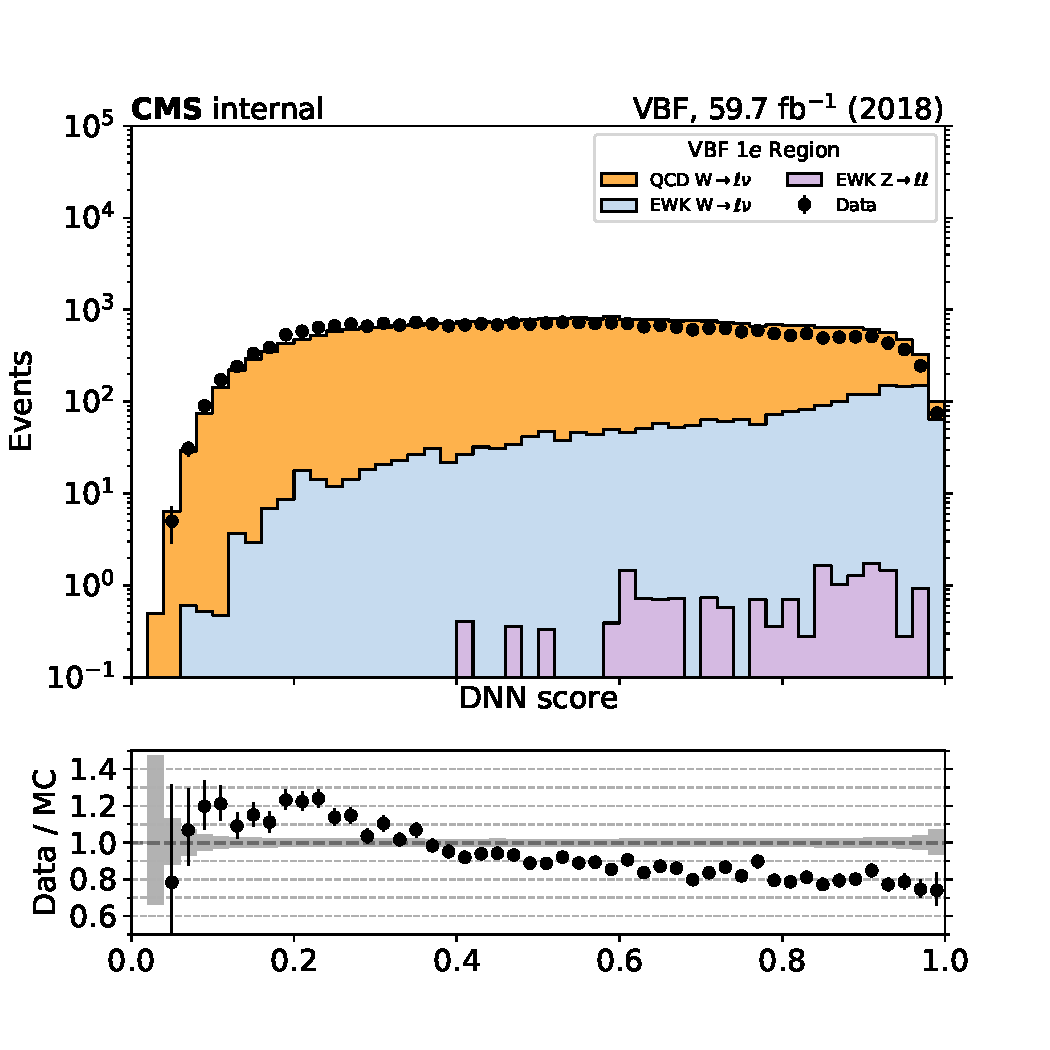
\includegraphics[width=0.45\textwidth]{VBFML/cr_1e_vbf_data_mc_particlenet_score_2018.pdf}
    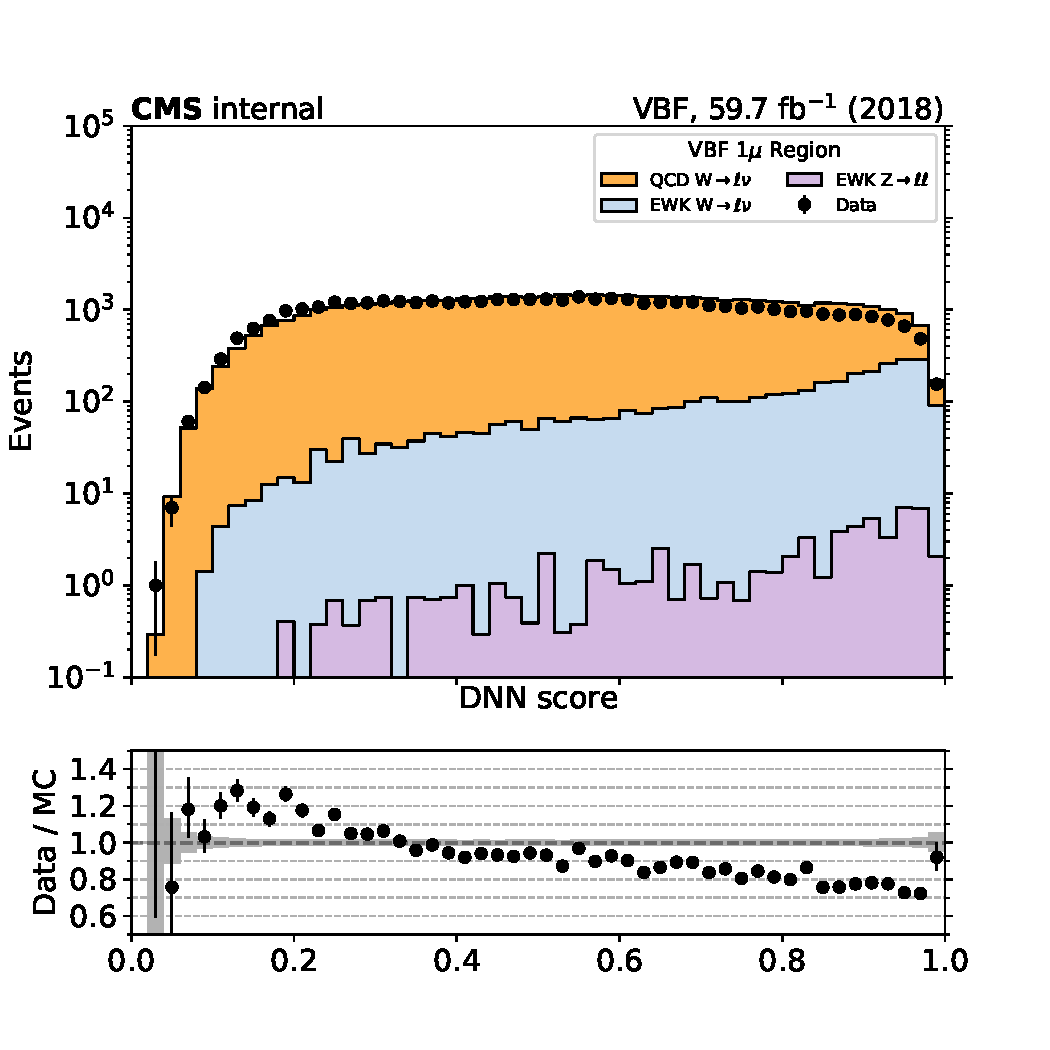
\includegraphics[width=0.45\textwidth]{VBFML/cr_1m_vbf_data_mc_particlenet_score_2018.pdf} \\
    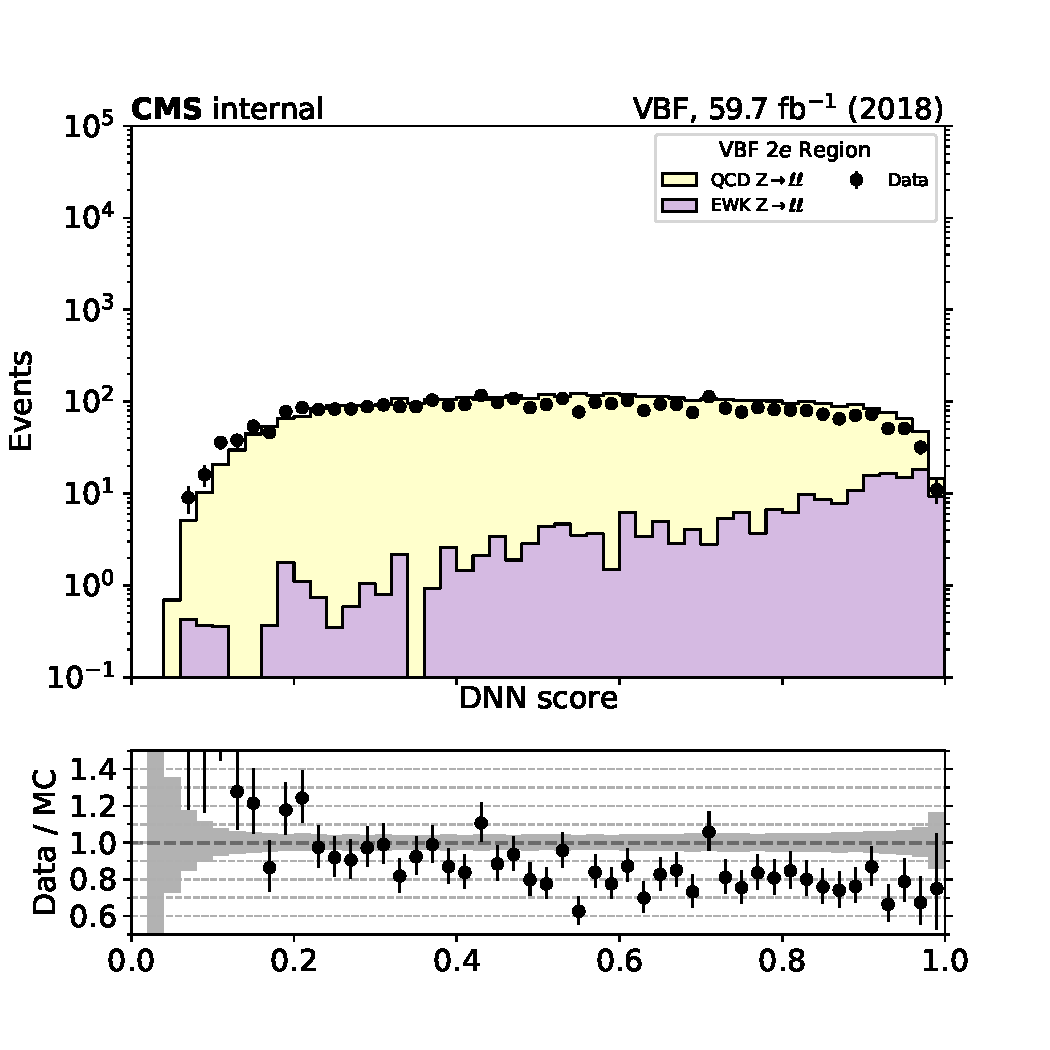
\includegraphics[width=0.45\textwidth]{VBFML/cr_2e_vbf_data_mc_particlenet_score_2018.pdf}
    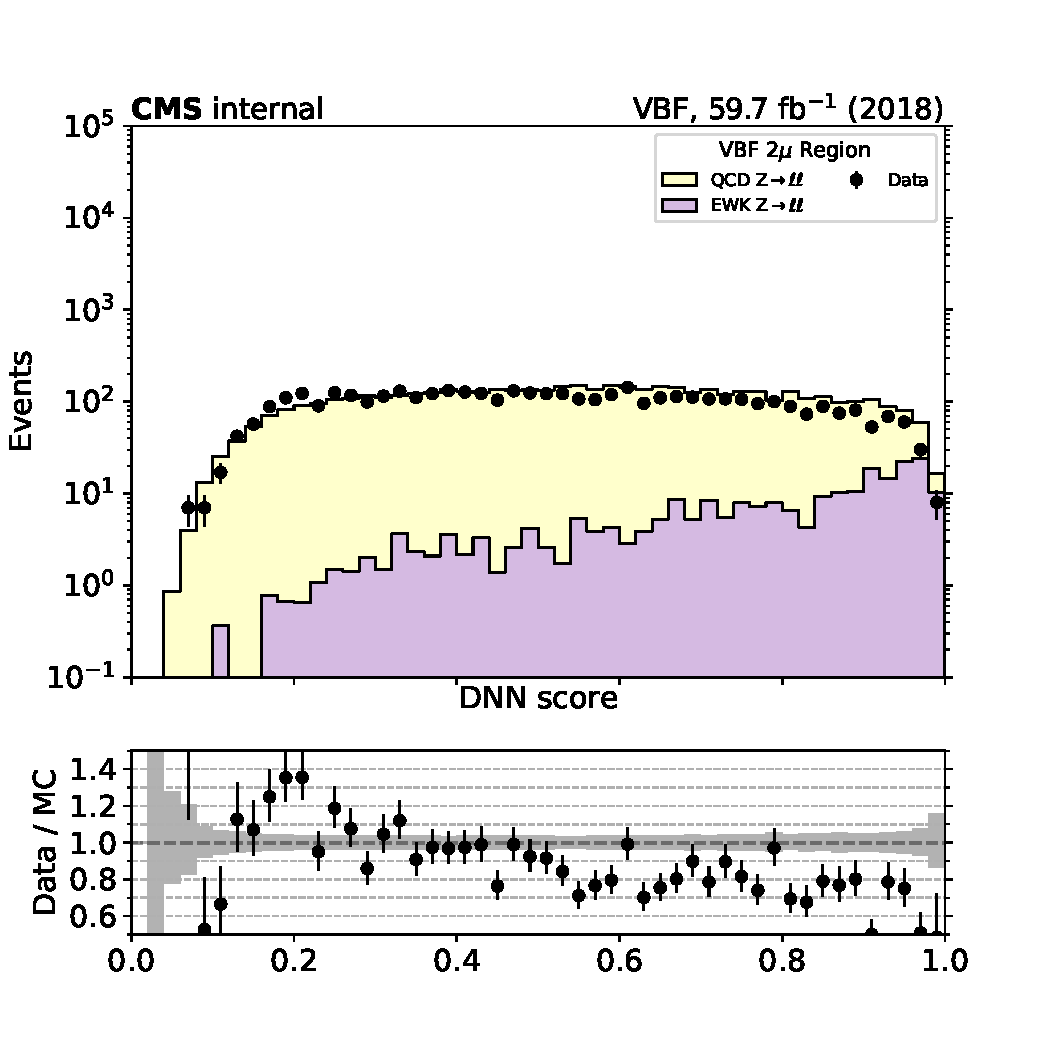
\includegraphics[width=0.45\textwidth]{VBFML/cr_2m_vbf_data_mc_particlenet_score_2018.pdf}
    \caption{Single electron (top left), single muon (top right), double electron (bottom left) and double muon (bottom right) control regions 
    as a function of the VBF-tagger score. The black markers in the top pad
    represent the observed data in each bin, and the stacks represent expected contributions from each process, obtained from simulation. The ratio pad
    at the bottom shows the ratio between the observed data and expected yields from simulation for each bin, and the grey band accounts for the statistical 
    uncertainties in the ratio.}
    \label{fig:single_lep_crs_vbfml}
\end{figure}

From Fig.~\ref{fig:single_lep_crs_vbfml}, a few interesting observations can be made:

\begin{itemize}
    \item Total expected (and observed) event yields do not have a significant shape as a function of VBF-tagger score. 
    This is expected because the event yields are dominated by the strong production of $\Vjets$, due to their larger cross section
    compared to the electroweak $\Vjets$ production modes.
    \item The electroweak $\Vjets$ contributions have an increasing shape with increasing VBF-tagger
    scores, which is also expected due to this process originating from VBF production of the corresponding vector boson.
    \item There is a trend in data to simulation ratio where the disagreement reaches to $\approx 20\%$. While this is not clearly
    understood, it is important to note that this trend appears consistently across different control regions. This allows this effect
    to approximately cancel out when the ratio of processes (transfer factors) are taken into account. It also supports the fact that
    the VBF-tagger predictions are not correlated with the reconstructed lepton, and only based on the hadronic activity within the event.  
\end{itemize}

To observe the partial cancellation mentioned in the last observation above, it is instructive to
look at ratios of $\Vjets$ processes (i.e. transfer factors) in different control regions.
These transfer factors as a function of VBF tagger score are shown in
Fig.~\ref{fig:cr_ratios_dnn_score}. The left-hand side plot shows the $\Zlljets$ to $\Wlvjets$ ratio,
where electron and muon channels are combined. It can be observed that there is reasonable agreement between
the ratios observed in data and predicted by simulation, within the statistical and systematical uncertainties.
The right-hand side plot shows the $\Zlljets$ to $\gamma$ + jets ratio, where some left-over disagreement in ratios
are observed. At the time of writing, this effect is not fully understood, but it should be noted that 
the simulation samples for $\Zlljets$ and $\Wlvjets$ are simulated at NLO in QCD, while the $\gamma$ + jets are
simulated in LO, with NLO corrections applied as a function of $\ptv$ and $\mjj$, as explained in Sec.~\ref{sec:nlo}.
Considering that all identified lepton and photon particles are removed from the input collection to the VBF tagger,
it is plausible that this difference can be playing a role in the shape of the predicted ratio in simulation. 

\begin{figure}[htbp]
    \centering
    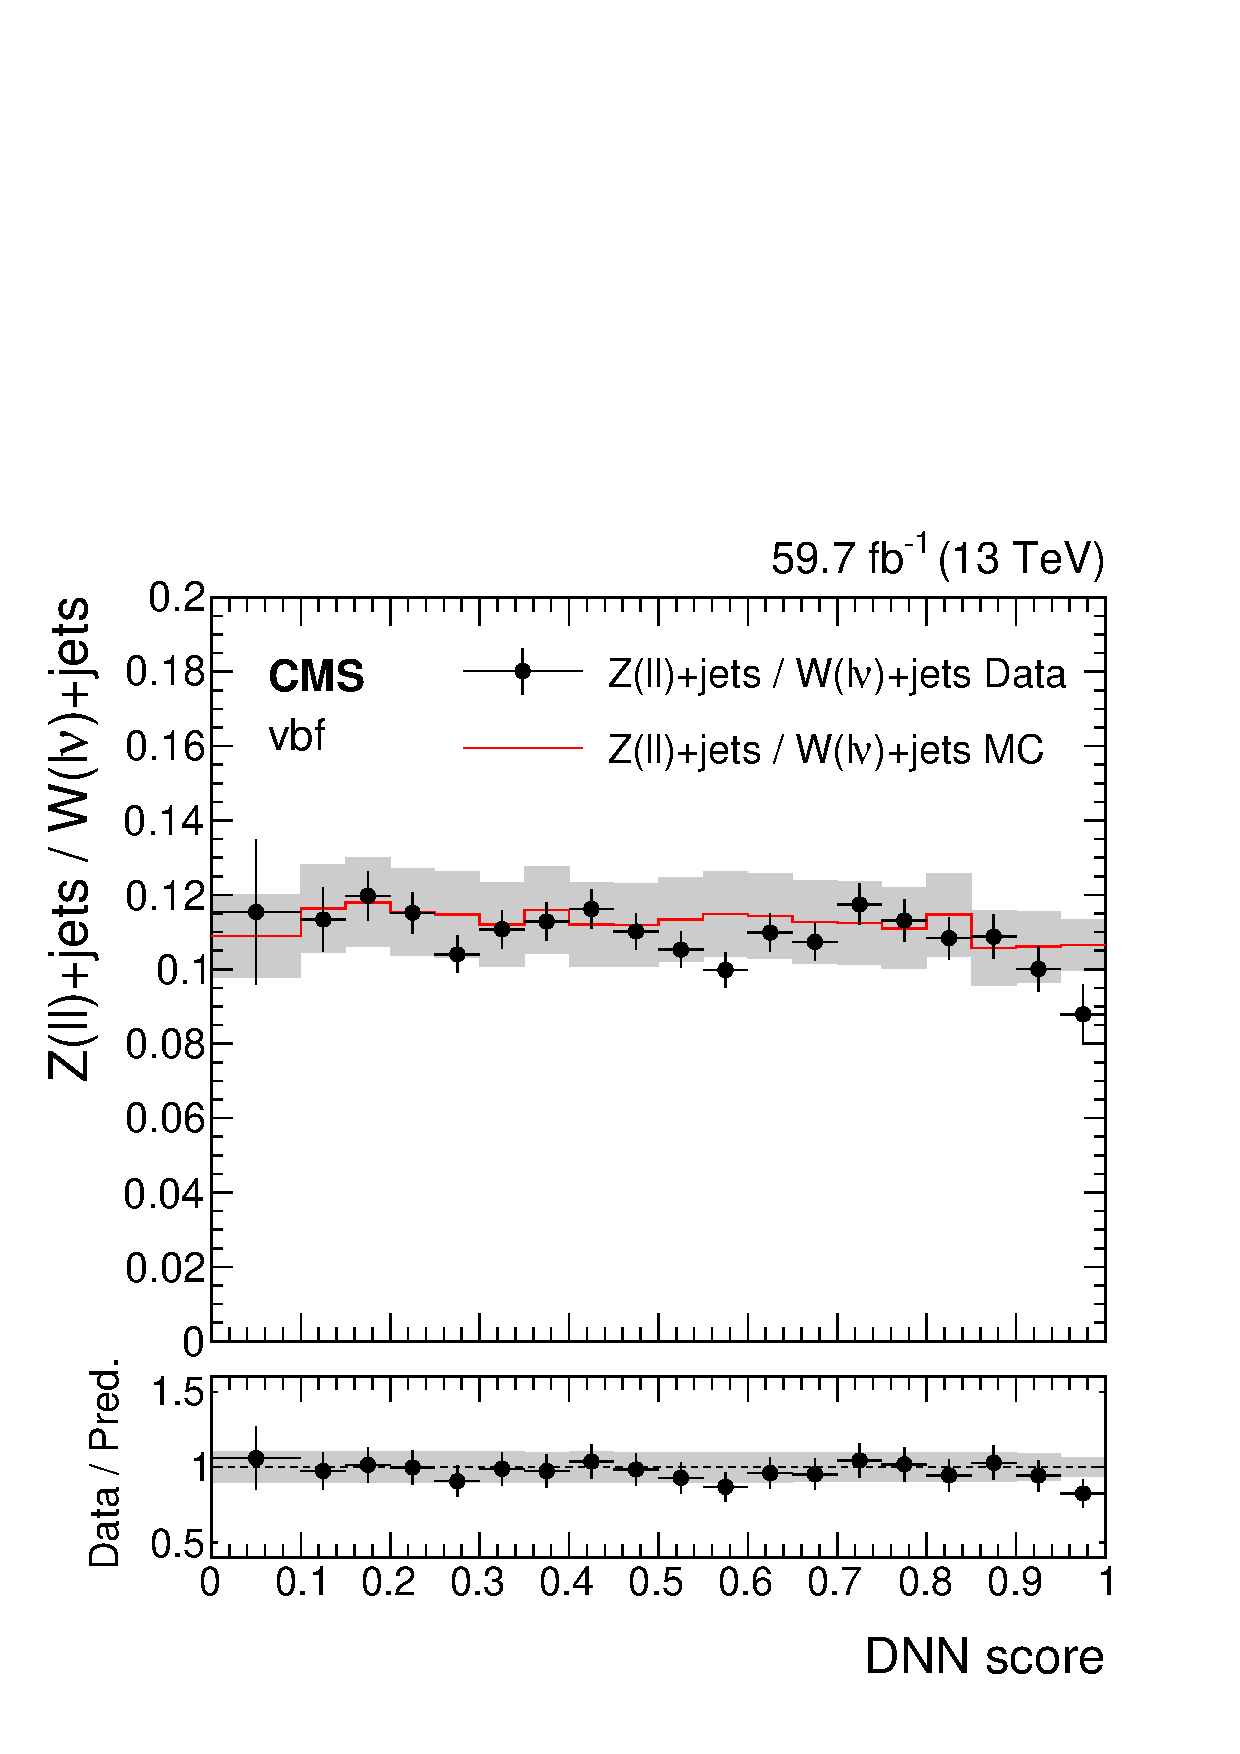
\includegraphics[width=0.45\textwidth]{VBFML/combined_combinedW_cat_vbf_2018_2018ratio.pdf}
    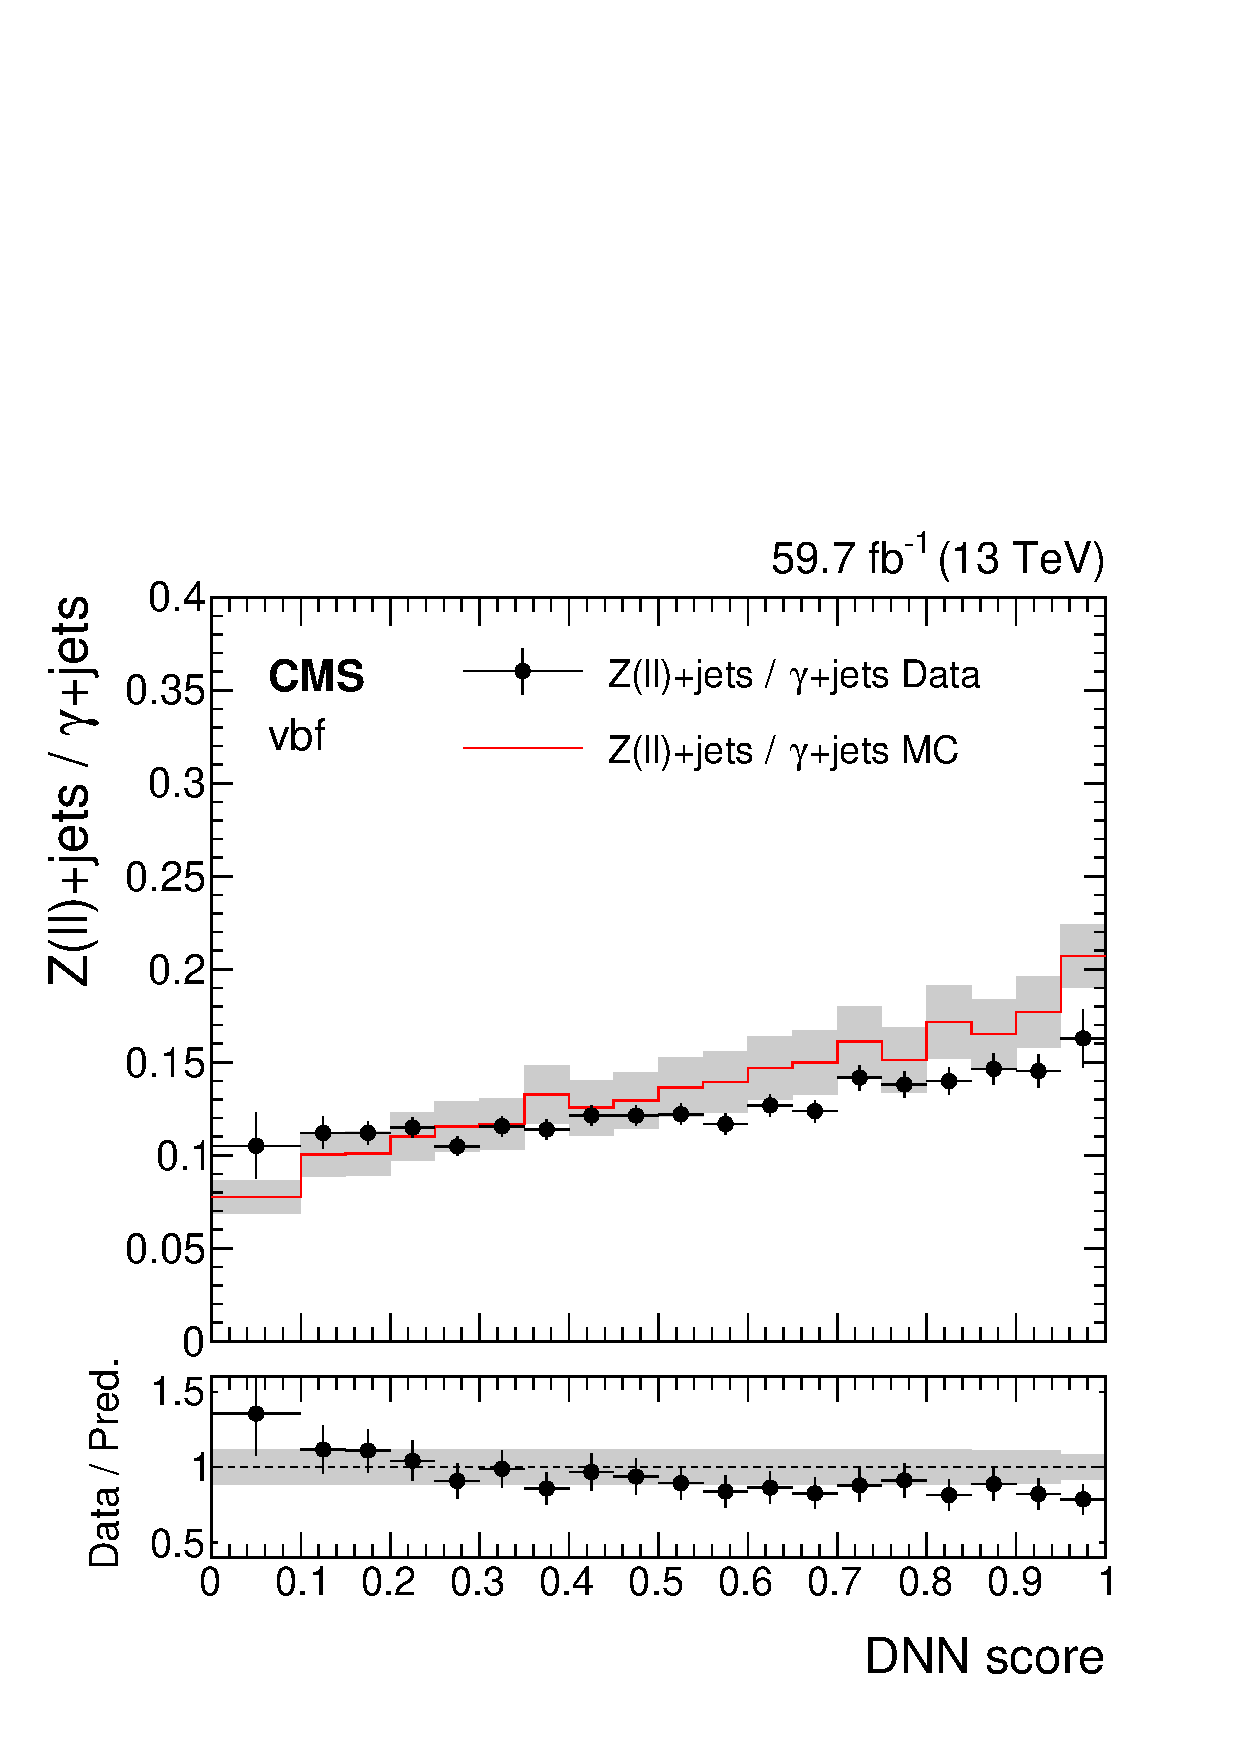
\includegraphics[width=0.45\textwidth]{VBFML/combined_gjets_cat_vbf_2018_2018ratio.pdf}
    \caption{Ratios of data and total simulation yields in $\Zlljets$ to $\Wlvjets$ ratio (left) and
    $\Zlljets$ to $\gamma$ + jets ratio (right), as a function of the VBF-tagger score. The black markers
    show the ratio in data observed in control regions, while the red line shows the ratio in simulated
    $\Vjets$ processes. The gray band represents the statistical and systematical uncertainties on the ratio.}
    \label{fig:cr_ratios_dnn_score}
\end{figure}

\subsection{Outlook}

Introducing powerful classifiers such as ParticleNet to enhance the sensitivity of the VBF $\hinv$ analysis
is definitely an interesting prospect. As mentioned in the previous sections, it is understood that ParticleNet can perform
better than a pure-$\mjj$ based classifier (i.e. Fig.~\ref{fig:ggh_vs_vbfh_roc}). However, the question of whether this
classifier can improve the statistical bounds on the $\brhinv$, hence enhancing the sensitivity of the analysis, is still open.

Application of the ParticleNet classifier to this analysis can be grouped into two different ways:

\begin{itemize}
    \item Perform the fit on the VBF-like score distribution, where the likelihood is described by Eq.~\ref{eq:fit_likelihood_func}.
    \item Perform a cut on the VBF-like score to reduce background (i.e. score $> X$), and perform the fit on $\mjj$ as before.
\end{itemize}

In both cases, the systematic uncertainties described in Sec.~\ref{subsec:sys_uncertainties} have to be recomputed. In the first case,
they need to be recomputed as a function of the ParticleNet score, while in the second case, they have to be recomputed for the high
VBF-like score phase space. Through further reduction of background using such a sophisticated classifier can in turn enhance the signal
to background ratio, resulting in an overall increase in the sensitivity of the analysis. With the Run3 data taking ongoing with Large
Hadron Collider (LHC) and the high luminosity stage (HL-LHC) on the horizon, much larger volumes of data will be able to analyze to probe
$\hinv$ decays, and the application of sophisticated classifiers such as ParticleNet remain an interesting variation of the analysis in
an attempt to enhance the sensitivity of the analysis.